\documentclass[]{article}
\usepackage{times}
\usepackage[margin=1in]{geometry}
\usepackage{algorithm2e}
\usepackage{dsfont}
\usepackage{amsmath}
\usepackage{hyperref}
\usepackage{pgf}
\usepackage{tikz}
\usepackage{subfig}
\usepackage{pgfplots}
\usepackage{filecontents}
\usepackage{listings}
\usepackage[round, sort, numbers]{natbib}

%opening
\title{CS3052 - Computational Complexity -\\Analysis of the Discrete Fourier Transform}
\author{ID:150013828}

\begin{document}

\maketitle

\section{Overview}
In this report, we give a look to each provided algorithm in turn. First, an \emph{a priori} analysis is provided for the worst-case time complexity of each - and subsequently, an empirical analysis of the average case of time complexity is provided (for \emph{two different machines}).
\\\\
Afterwards, an analysis of the threshold for which FFT outperforms naive DFT is described in section \ref{sec:threshold}.
\\\\
In case there is any doubt: \emph{task 1} is mapped to sections \ref{sec:dft-worst} and \ref{sec:fft-worst}; \emph{task 2 and 3} are mapped to sections \ref{sec:dft-average} and \ref{sec:fft-average} respectively; and \emph{task 4} is mapped to section \ref{sec:threshold}.

\section{Setup}
In order to benchmark the functions provided, the framework \emph{JMH}\cite{ref:jmh} is used. An article from \emph{Oracle}\cite{ref:oracle-benchmarking} outlines why it is preferable to use JMH over naive methods like measuring time before and after, etc..
\\\\
The provided benchmark runner prepares random inputs upon every startup and runs the benchmark for the specified number of iterations; \emph{forking} each set of iterations to help alleviate any scheduling bias on the OS' part; and performing a \emph{warmup} before the main iteration phase.
\\\\
In order to run the benchmarks exactly as done so for this set of analysis (this project requires \emph{Maven}), run:\\\\
\begin{minipage}[!h]{\linewidth}
	\begin{lstlisting}[frame=single,language=bash]
	mvn clean install
	java -cp target/benchmarks.jar uk.ac.st_andrews.Benchmarker
	\end{lstlisting}
\end{minipage}

This runs the benchmarker with the default settings - and should run for approximately an hour, regardless of the machine. The benchmarking framework does not output anything to \emph{stdout} while it is running in file output mode, unfortunately - so the terminal will remain empty for as long as the benchmark runs.
\\\\
All code is in the \texttt{src} directory. All \emph{tex} files in \texttt{tex}, and all CSV files, XLS workbooks etc. are in \texttt{tex/csv}.

\section{DFT Analysis}\label{sec:dft}
\subsection{Worst Case Time Complexity}\label{sec:dft-worst}
First, the algorithm in question is shown in pseudocode in algorithm \ref{alg:dft}.

\begin{algorithm}[h]
	\KwIn{$x_0, x_1, ..., x_{N-1} : x \in \mathds{C}$}
	$Y = \verb|the empty list|$\\
	\For{$j = 0$; $j < N$}{
		$Y_j = 0$\\
		\For{$k = 0$; $k < N$}{
			$z = e^{-2jk\pi i / N} = \cos(\frac{-2jk\pi}{N}) + i \sin(\frac{-2jk\pi}{N})$\\
			$Y_j \leftarrow Y_j + zx_k$\\
			$k \leftarrow k + 1$\\
		}
		$j \leftarrow j + 1$\\
	}
	\Return{X}\\
\caption{The naive DFT algorithm\label{alg:dft}}
\end{algorithm}

For this algorithm, the worst-case time complexity is quite clear. As can be seen in the pseudocode, the algorithm contains one \emph{for-loop} nested inside another - both of which iterate $N$ times, where $N$ is the size of the input list. Hence, the total number of evaluations of the inner loop is $N^2$.
	
Knowing that the code within the loop does not break at an early point - we can say that the time taken for an input list of size $n$, $T(n)$, is at the least, proportional to $n^2$. The evaluation of the inner loop will be of a constant factor, this is because the operations, $\sin$, $\cos$, addition, multiplication etc. will always take the same time within this context. I.e. we do not use arbitrary precision floating point numbers, the size is \emph{fixed}. So, it is reasonable to say that the inner loop is of a constant order complexity.

Now we know that: the inner loop will always run $N^2$ times; and that the evaluation of the inner loop is of the order $O(1)$ with respect to a single element of the input list. With all of these facts in mind, it is reasonable to assume that the naive DFT algorithm is of the order $O(n^2)$, where $n$ is the length of the input list. Not only this, but the average case, and even the best case, should be asymptotically the same as the worst case - this is because there is no room for pathological behaviour in the algorithm, it \emph{always} runs the inner loop $N^2$ times. That is to say, the algorithm is $\Omega(n^2)$, and $O(n^2) \Rightarrow \Theta(n^2)$.

\subsection{Average Case Analysis}\label{sec:dft-average}

\begin{figure}[!htbp]
	\centering
	\begin{minipage}[b]{0.4\textwidth}
		\begin{tikzpicture}
		\begin{axis}[ xmin=0, ymin=0, xlabel=Input Length, ylabel=Time ($\mu$s), legend style={at={(1,-0.1)},anchor=north} ]
		\addplot table [ignore chars=\%, x=Param: inputLength, y=Score, col sep=comma] {csv/pc1-result-dft.csv};
		\addlegendentry{PC1}
		\end{axis}
		\end{tikzpicture}
		\caption{Naive DFT - PC1\label{fig:compar1}}
	\end{minipage}
	\hfill
	\begin{minipage}[b]{0.4\textwidth}
		\begin{tikzpicture}
		\begin{axis}[ xmin=0, ymin=0, xlabel=Input Length, ylabel=Time ($\mu$s), legend style={at={(1,-0.1)},anchor=north} ]
		\addplot table [ignore chars=\%, x=Param: inputLength, y=Score, col sep=comma] {csv/pc2-result-dft.csv};
		\addlegendentry{PC2}
		\end{axis}
		\end{tikzpicture}
		\caption{Naive DFT - PC2\label{fig:compar2}}
	\end{minipage}
\end{figure}

Further analysis is produced, using \emph{Microsoft Excel 2013's} polynomial curve fitting feature (for polynomials of order two). It calculates the coefficients of a second-order polynomial with impressive \emph{r-squared} values of 0.9999 each.
\begin{figure}[!htbp]
	\centering
	\begin{minipage}[b]{0.4\textwidth}
		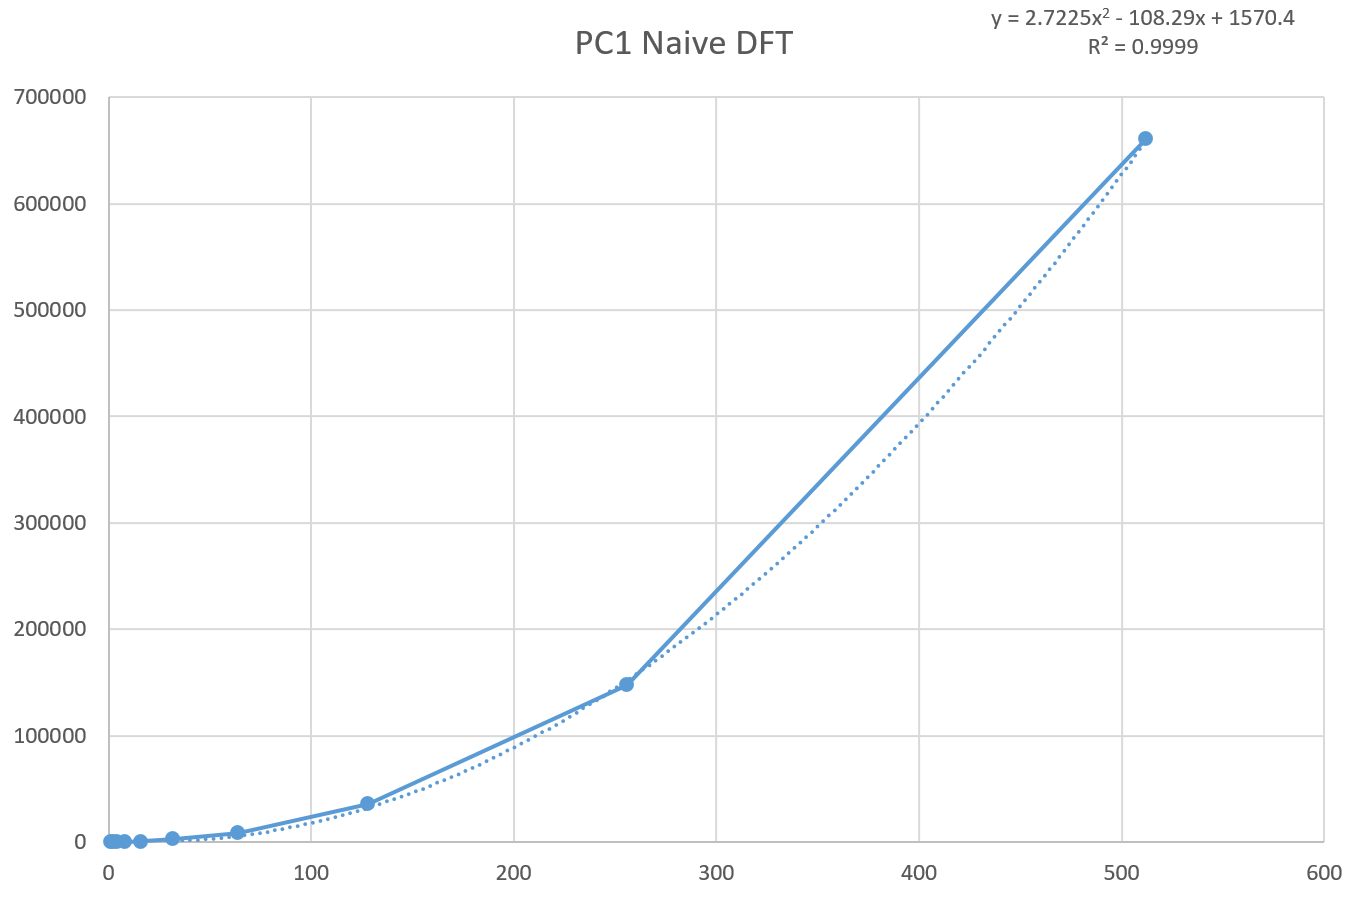
\includegraphics[width=\linewidth]{csv/pc1-dft-fit}
		\caption{Naive DFT - PC2\label{fig:pc1-dft-fit}}
	\end{minipage}
	\hfill
	\begin{minipage}[b]{0.4\textwidth}
		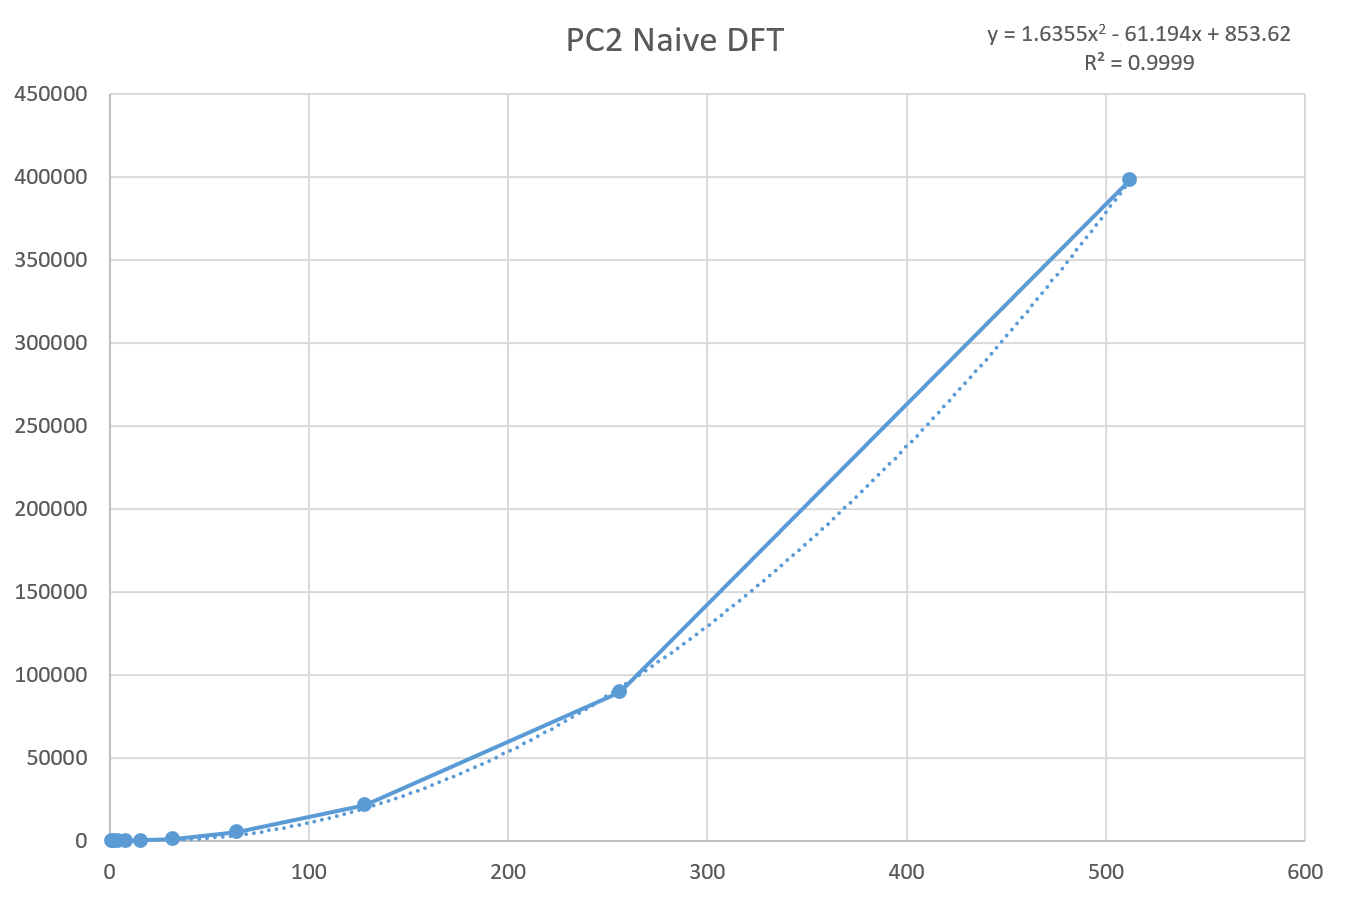
\includegraphics[width=\linewidth]{csv/pc2-dft-fit}
		\caption{Naive DFT - PC2\label{fig:pc2-dft-fit}}
	\end{minipage}
\end{figure}

We can be confident that, given the measured data, the curve $y = 2.7225x^2 + 108.29x + 1570.4$ approximates the time taken for PC1 to calculate the naive DFT of an arbitrary number of inputs. Likewise, $y = 1.6355x^2 + 61.194x + 853.62$ approximates the time taken for PC2.

\section{FFT Analysis}\label{sec:fft}

\subsection{Worst Case Time Complexity}\label{sec:fft-worst}
As before, the algorithm in question is shown in pseudocode in algorithm \ref{alg:fft}.
\begin{algorithm}[h]
	\KwIn{$x_0, x_1, ..., x_{N-1} : x \in \mathds{C}$}
	\If{N = 1}{
		\Return $x_0$
	}
	\If{$N$ is not even}{
		\Return error: $N$ should be a power of two
	}
	$q = \verb|FFT(all even terms in input list)|$\\
	$r = \verb|FFT(all odd terms in input list)|$\\
	$Y = \verb|the empty list|$\\
	\For{$k = 0$; $k < N/2$}{
		$z = e^{-2k\pi i / N} = \cos(\frac{-2k\pi}{N}) + i \sin(\frac{-2k\pi}{N})$\\
		$Y_k = q_k + zr_k$\\
		$Y_{k + N/2} = q_k - zr_k$\\
		$k \leftarrow k + 1$\\
	}
	\Return Y
	\caption{The Fast Fourier Transform (FFT) algorithm
\label{alg:fft}}
\end{algorithm}

In order to analyse the complexity of the FFT algorithm, we will apply the \emph{master theorem} - as shown in the lectures of this module. The motivation to do so is that the algorithm is recursive, and may be expressed as a recurrence relation. First, we must show what that recurrence relation is, and then figure out which case of the master theorem it lies in.
\\\\
The time taken for the FFT algorithm is proportional to the following recurrence relation:
$$T(n) = 2T(\frac{n}{2}) + \Theta(n)$$
where $T(n)$ is the time taken for an input list of size $n$. The reasoning behind this is clear from the pseudocode in algorithm \ref{alg:fft}. The first term of the recurrence relation, $2T(\frac{n}{2})$ arises because, as algorithm \ref{alg:fft} shows, two recursions of itself are computed on an input which is \emph{half} the size of the original. I.e. $\verb|FFT|$ is computed for all items in the input with an even index, and the same again for all items with an odd index.

After the recursion, computation is done to find multiple \emph{roots of unity}. Similarly to the case of algorithm \ref{alg:dft}, we shall say that this takes a constant amount of time to evaluate, as it runs a fixed set of operations on an item of data with a fixed size. This computation happens precisely $N/2$ times, except in the very specific case that $N = 1$ which is constant. However this special case still applies to the lower bound of $\Omega(n)$ because it is only the case when $n = 1$ and $\Omega(n) = \Omega(1)$ anyway. Hence, the second term - the computational overhead after that of recursion - is of the order $\Omega(n)$, and $O(n) \Rightarrow \Theta(n)$; bringing us to the recurrence relation shown.
\\\\
Given this recurrence relation, we must next find out which case of the master theorem (one, two, or three) applies.
\paragraph{Case 1}
For a recurrence relation of the form...
$$T(n) = aT(\frac{n}{b}) + f(n)$$
...the following statement must also apply in case one:
\[
f(n) = O(n^{\log_b{a - \epsilon}}) \text{ where } \epsilon > 0
\]
We know the values of $a$ and $b$ to both be $2$, it is easy to see. But, the second term, $\Theta(n)$ does not apply to case one because $\Theta(n) = O(n^{\log_2{2 - \epsilon}})$ is only the case when $\epsilon = 0$.

\paragraph{Case 2}
Next, the following statement must apply in case two:
\[
f(n) = O(n^{\log_b{a}}\log^k{n}) \text{ for some } k \geq 0
\]
Using the known values of $a$ and $b$, and selecting a value of $k = 0$, we get:
\[
O(n(\log{n})^0) = O(n)
\]
showing that our second term, $\Theta(n)$ satisfies case two.

\paragraph{Conclusion}
For case two of the master theorem, the complexity is asymptotically tightly bound as $\Theta(n^{log_b{a}}\log^{k + 1}n)$. Substituting the values from the above discussion, $a = 2$, $b = 2$, $k = 0$ we find that the complexity for FFT is $$\Theta(n\log{n})$$

\subsection{Average Case Analysis}\label{sec:fft-average}
\begin{figure}[!htbp]
	\centering
	\begin{minipage}[b]{0.4\textwidth}
		\begin{tikzpicture}
		\begin{axis}[ xmin=0, ymin=0, xlabel=Input Length, ylabel=Time ($\mu$s), legend style={at={(1,-0.1)},anchor=north} ]
		\addplot table [ignore chars=\%, x=Param: inputLength, y=Score, col sep=comma] {csv/pc1-result-fft.csv};
		\addlegendentry{PC1}
		\end{axis}
		\end{tikzpicture}
		\caption{FFT - PC1\label{fig:compar3}}
	\end{minipage}
	\hfill
	\begin{minipage}[b]{0.4\textwidth}
		\begin{tikzpicture}
		\begin{axis}[ xmin=0, ymin=0, xlabel=Input Length, ylabel=Time ($\mu$s), legend style={at={(1,-0.1)},anchor=north} ]
		\addplot table [ignore chars=\%, x=Param: inputLength, y=Score, col sep=comma] {csv/pc2-result-fft.csv};
		\addlegendentry{PC2}
		\end{axis}
		\end{tikzpicture}
		\caption{FFT - PC2\label{fig:compar4}}
	\end{minipage}
\end{figure}

It is a little more tricky to figure out whether or not these data sets actually correspond to a function proportional to $n\log n$ using \emph{Microsoft Excel}. However, if the data is plotted like so in figure \ref{fig:compar8} - where the y-axis now represents $\frac{T}{n}$ (dividing \emph{both sides} by n) we can now attempt to fit the data against a logarithmic curve. Excel \emph{can} do this. If the relationship is satisfactorily logarithmic, then the time taken should also be satisfactorily proportional to $n\log n$.
\begin{figure}[!htbp]
	\begin{center}
		\begin{tikzpicture}
		\begin{axis}[ xmin=0, ymin=0, xlabel=Input Length ($n$), ylabel=($\mu$s$n^{-1}$), legend style={at={(1,-0.1)},anchor=north} ]
		\addplot table [ignore chars=\%, x=Param: inputLength, y=score per input length, col sep=comma] {csv/pc1-result-fft.csv};
		\addlegendentry{PC1}
		\addplot table [ignore chars=\%, x=Param: inputLength, y=score per input length, col sep=comma] {csv/pc2-result-fft.csv};
		\addlegendentry{PC2}
		\end{axis}
		\end{tikzpicture}
		\caption{$\frac{T}{N}$ against input length $N$\label{fig:compar8}}
	\end{center}
\end{figure}

\begin{figure}[!htbp]
	\centering
	\begin{minipage}[b]{0.4\textwidth}
		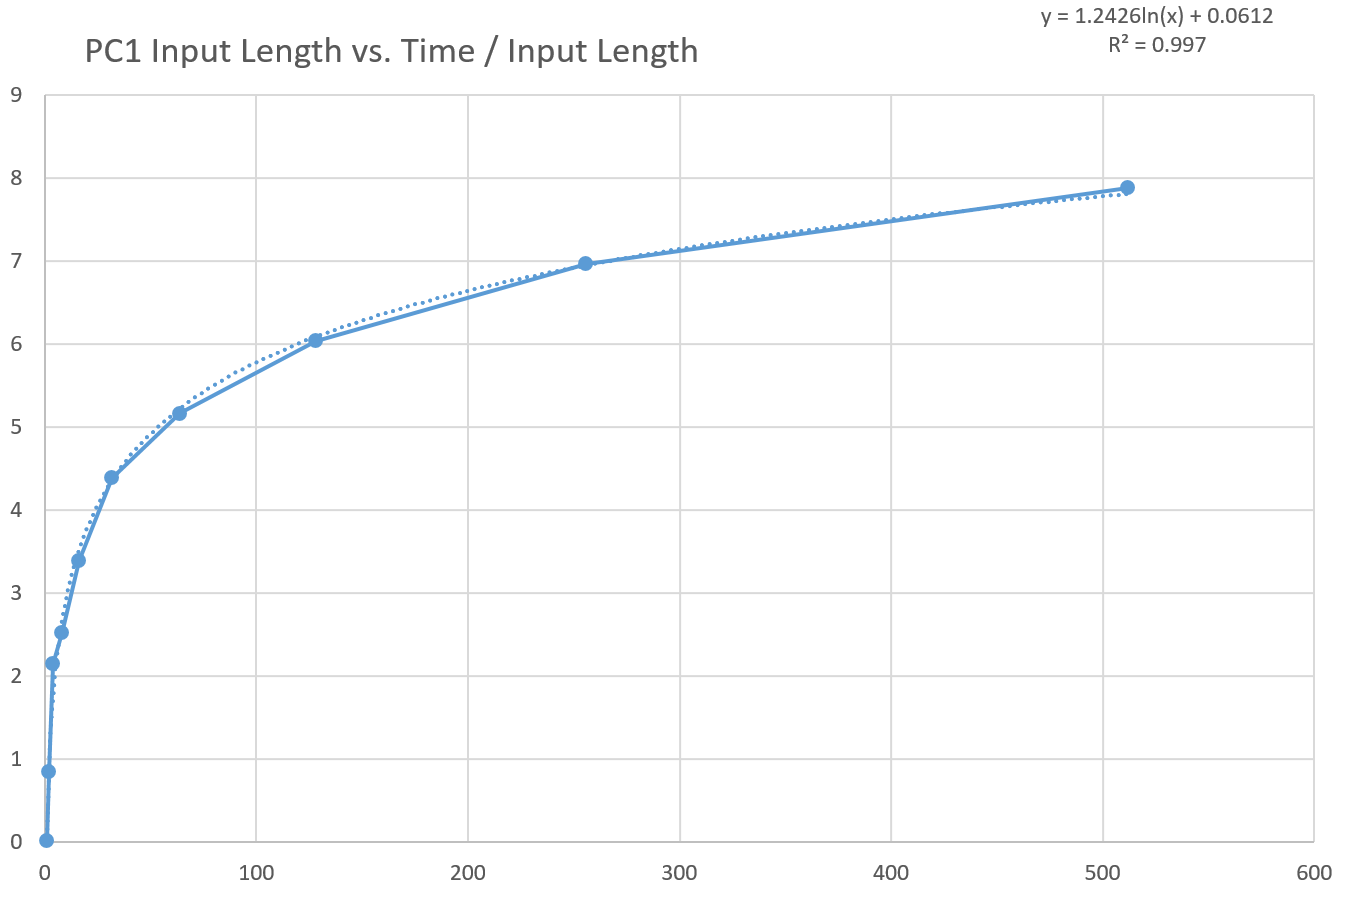
\includegraphics[width=\linewidth]{csv/pc1-fft-fit}
		\caption{Fitting FFT results against a logarithmic curve - PC1\label{fig:pc1-fft-fit}}
	\end{minipage}
	\hfill
	\begin{minipage}[b]{0.4\textwidth}
		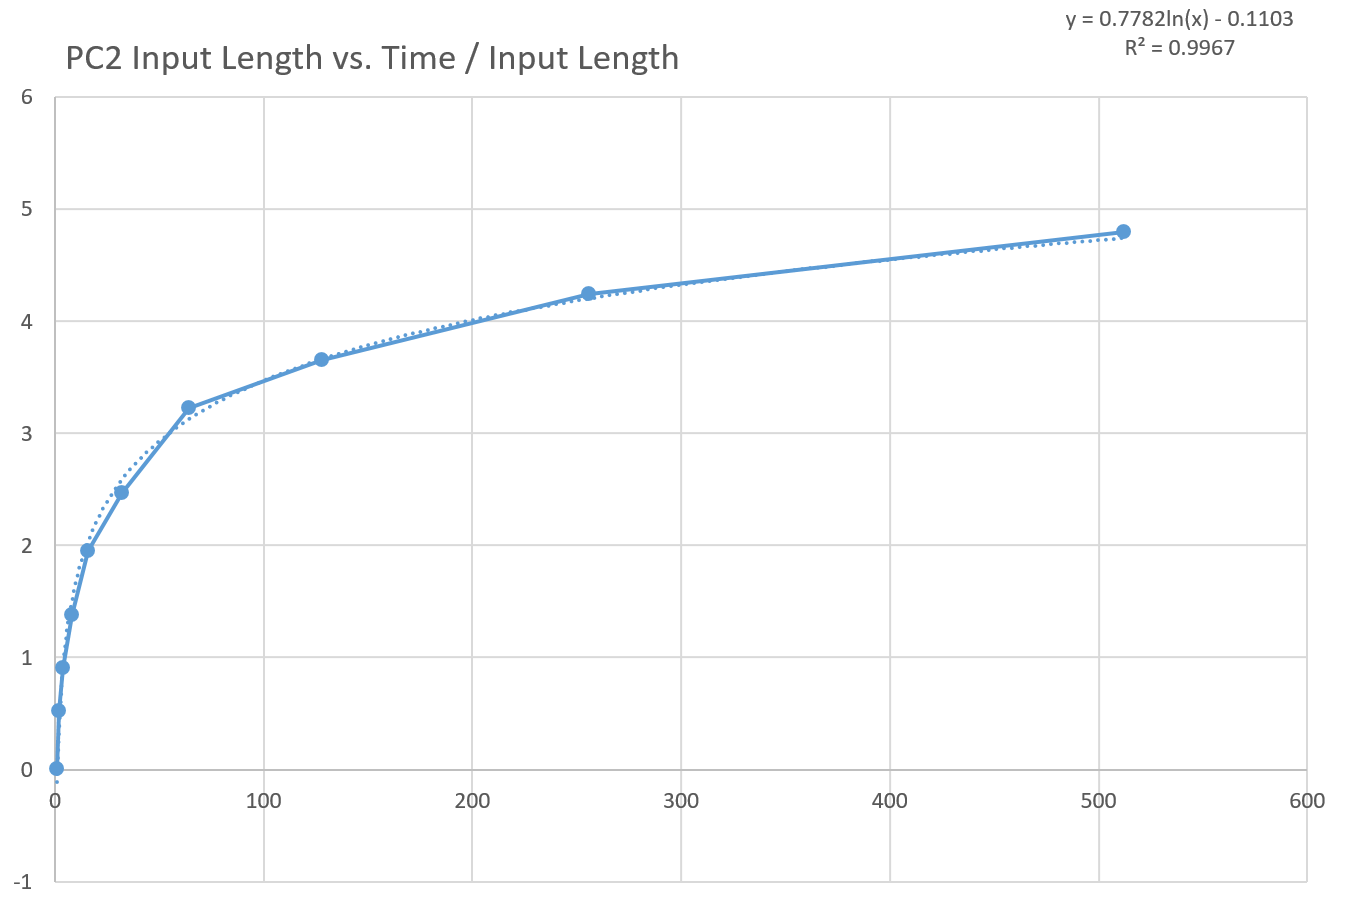
\includegraphics[width=\linewidth]{csv/pc2-fft-fit}
		\caption{Fitting FFT results against a logarithmic curve - PC2\label{fig:pc2-fft-fit}}
	\end{minipage}
\end{figure}

As before, \emph{Excel} can calculate the coefficients, $a$ and $b$ of a logarithmic equation of the form $y = a\ln(x) + b$.

\emph{Excel} calculates $y = 1.246\ln(x) + 0.0612$ as an approximation for the relationship of PC1's data. And again, $y = 0.7782\ln(x) + 0.1103$ for PC2. Both of these approximations also have a high $R^2$ value, as with section \ref{sec:dft-average} - inspiring confidence. Of course, to be on the same terms as what we're expecting we can use the equivalent forms $y = ln(x) = \frac{\log_2{x}}{\log_2{e}}$. Thus, the approximations are also $y = \frac{1.246}{\log_2{e}}\log_2{x} + 0.0612$ and $y = \frac{0.7782}{\log_2{e}}\log_2{x} + 0.1103$ respectively.

Finally, multiply by $n$ again to get the complete approximation:
$$\verb|PC1: |n(\frac{1.246}{\log_2{e}}\log_2{n} + 0.0612)$$
$$\verb|PC2: |n(\frac{0.7782}{\log_2{e}}\log_2{n} + 0.1103)$$
\section{The Value of the DFT/FFT Threshold}\label{sec:threshold}
For the sake of comparison, the two average cases described in sections \ref{sec:dft-average} and \ref{sec:fft-average} are shown here in the same plot (figure \ref{fig:compar7}). It is easy to see that, in the asymptotic case, FFT will win against DFT - all things continuing the shown trend. Given the name, however, this is somewhat expected.
\begin{figure}
	\begin{center}
		\begin{tikzpicture}
		\begin{axis}[ xmin=0, ymin=0, xlabel=Input Length, ylabel=Time ($\mu$s), legend style={at={(1,-0.1)},anchor=north} ]
		\addplot table [ignore chars=\%, x=Param: inputLength, y=Score, col sep=comma] {csv/pc1-result-dft.csv};
		\addlegendentry{PC1 DFT}
		\addplot table [ignore chars=\%, x=Param: inputLength, y=Score, col sep=comma] {csv/pc1-result-fft.csv};
		\addlegendentry{PC1 FFT}
		\addplot table [ignore chars=\%, x=Param: inputLength, y=Score, col sep=comma] {csv/pc2-result-fft.csv};
		\addlegendentry{PC2 FFT}
		\addplot table [ignore chars=\%, x=Param: inputLength, y=Score, col sep=comma] {csv/pc2-result-dft.csv};
		\addlegendentry{PC2 DFT}
		\end{axis}
		\end{tikzpicture}
		\caption{DFT and FFT for PC1 and PC2\label{fig:compar7}}
	\end{center}
\end{figure}

\begin{figure}
	\begin{center}
		\begin{tikzpicture}
		\begin{axis}[domain=-8:2, restrict y to domain=0:25, xmin=0, xmax=4, ymin=0, xlabel=Input Length, ylabel=Time ($\mu$s), legend style={at={(1,-0.1)},anchor=north} ]
		\addplot table [ignore chars=\%, x=Param: inputLength, y=Score, col sep=comma] {csv/pc1-result-dft.csv};
		\addlegendentry{PC1 DFT}
		\addplot table [ignore chars=\%, x=Param: inputLength, y=Score, col sep=comma] {csv/pc1-result-fft.csv};
		\addlegendentry{PC1 FFT}
		\addplot table [ignore chars=\%, x=Param: inputLength, y=Score, col sep=comma] {csv/pc2-result-fft.csv};
		\addlegendentry{PC2 FFT}
		\addplot table [ignore chars=\%, x=Param: inputLength, y=Score, col sep=comma] {csv/pc2-result-dft.csv};
		\addlegendentry{PC2 DFT}
		\end{axis}
		\end{tikzpicture}
		\caption{showing the \emph{threshold} for which FFT outperforms DFT for PC1 and PC2\label{fig:compar10}}
	\end{center}
\end{figure}
As one can immediately see in figure \ref{fig:compar10}, the threshold value, if it exists, must be very small. We need to look closer. In fact, FFT was measured to be faster than DFT for \emph{all} cases. The threshold is the base case itself. FFT is flat out \emph{better}!

\paragraph{Note About Per-Machine Performance} What I expected to happen, was that there would be some perceivable threshold value, and that one would be able to approximate it by equating the two approximations for time with input size obtained in sections \ref{sec:dft-average} and \ref{sec:fft-average}. Also, my expectation was that the differing machine performance would change the value of the threshold. However, as has been illustrated for the two machines used (see \ref{fig:specs} for more information about the hardware runnning these benchmarks) FFT is \emph{always} faster. 

But, as shown in figure \ref{fig:compar6}, the different machine specs does give rise to difference coefficients in the approximation of time with input (see \ref{sec:dft-average} and \ref{sec:fft-average})
\begin{figure}
	\centering
	\begin{minipage}[b]{0.4\textwidth}
		\begin{tikzpicture}
		\begin{axis}[ xmin=0, ymin=0, xlabel=Input Length, ylabel=Time ($\mu$s), legend style={at={(1,-0.1)},anchor=north} ]
		\addplot table [ignore chars=\%, x=Param: inputLength, y=Score, col sep=comma] {csv/pc1-result-dft.csv};
		\addlegendentry{PC1}
		\addplot table [ignore chars=\%, x=Param: inputLength, y=Score, col sep=comma] {csv/pc2-result-dft.csv};
		\addlegendentry{PC2}
		\end{axis}
		\end{tikzpicture}
		\caption{Naive DFT for PC1 and PC2\label{fig:compar5}}
	\end{minipage}
	\hfill
	\begin{minipage}[b]{0.4\textwidth}
		\begin{tikzpicture}
		\begin{axis}[ xmin=0, ymin=0, xlabel=Input Length, ylabel=Time ($\mu$s), legend style={at={(1,-0.1)},anchor=north} ]
		\addplot table [ignore chars=\%, x=Param: inputLength, y=Score, col sep=comma] {csv/pc1-result-fft.csv};
		\addlegendentry{PC1}
		\addplot table [ignore chars=\%, x=Param: inputLength, y=Score, col sep=comma] {csv/pc2-result-fft.csv};
		\addlegendentry{PC2}
		\end{axis}
		\end{tikzpicture}
		\caption{FFT for PC1 and PC2\label{fig:compar6}}
	\end{minipage}
\end{figure}

\begin{figure}
	\begin{center}
		\begin{tabular}{ | c | c | c | }
			\hline
			specification & PC1 Value & PC2 Value \\
			\hline
			CPU & x86\_64 Intel(R) i7-4712HQ @ 2.30GHz & x86\_64 Intel(R) i5-3470S @ 2.90GHz\\
			\hline
			RAM & 16GB = 2 $\times$ 8GB @ 1600MHz DDR3 & 8GB - unknown clock rate and number of sticks\\ 
			\hline
			OS & Ubuntu \emph{xenial} 16.04.2 & Fedora release 24\\
			\hline
			Java Version & 1.8.0\_121 & 1.8.0\_121\\
			\hline
		\end{tabular}
	\end{center}
	\caption{relevant system specifications used in provided analysis\label{fig:specs}}
\end{figure}


\section{Evaluation}
I think that the benchmarks outlined here provide fairly detailed analysis, albeit that the number of forks, warmups, and iterations could be higher to increase confidence that the data is properly representative (I had limited time, once I had created the benchmarker). I would like to have done more with curve fitting, perhaps in something more powerful than \emph{Microsoft Excel 2013}. The way I approach finding an approximation of the time taken for FFT is a rather \emph{visual} approach to \emph{decomposition} - however, I personally do not know of a sufficient method to fit curves of the form $n\log{n}$.
\\\\
I would like to have experimented with more input points, however the benchmarking time would return "Infinity" for input lists of approximately 1000 in length. I suspect that the time taken to measure has gone completely out of the time unit's precision range in this case.
\\\\
However, one of the most annoying facts about this submission is that the measured results are not automatically fed into a specific set of analysis - such as that which is seen in the report. Indeed, I had to manually move around some of the columns in the output CSV files in order for the given plots here to display in latex (by CSV input). I believe something like \emph{R} or \emph{MATLAB} would be perfect for alleviating this.
\bibliography{ref}
\bibliographystyle{apalike}

\end{document}
